\chapter[Structuring Machine Learning Projects]{Structuring Machine \\Learning Projects}

%%%
\section{ML Strategy}


%%%%
\subsection{Introduction to ML Strategy}

\subsubsection{Why ML Strategy}

为了提高深度学习系统的准确性,可以尝试以下方法:

\begin{itemize}
    \item 收集更多数据。
    \item 收集更多样化的训练集。
    \item 训练更多轮数。
    \item 尝试不同的优化算法(例如 Adam)。
    \item 添加正则化方法。
    \item 改变网络架构(激活函数、隐藏单元数量等)。
\end{itemize}

这些方法在什么情况下适合使用,是本章主要探讨的内容。

\subsubsection{Orthogonalization}
\index{Orthogonalization}

\textbf{正交化(Orthogonalization)}是指调整超参数以实现特定效果的过程。
在正交化中,每个控制参数只执行特定任务,不影响其他控制参数,做到“互不干扰”。

对于监督学习系统来说,要表现良好,通常需要调整系统参数以确保下面的四个条件成立:

\begin{enumerate}
    \item 在成本函数上很好地拟合训练集(尽可能接近甚至超过人类水平)。
    \item 在成本函数上很好地拟合开发集。
    \item 在成本函数上很好地拟合测试集。
    \item 在现实世界的真实数据中表现良好。
\end{enumerate}


%%%%
\subsection{Setting Up your Goal}

\subsubsection{Single Number Evaluation Metric}

单一的、明确的、可量化的评估指标可以帮助你快速了解你的模型的性能。
确定一个\textbf{单一数字评估指标(Single Number Evaluation Metric)}是评估深度学习系统性能的重要一步,
有了这个明确的量化标准,可以更方便地比较不同模型的性能,并不断对系统进行迭代改进。

通常,这个指标可以是准确率、mAP、Artificial Analysis Quality Index(人工分析质量指数)等。
在有些情况下,简单的准确率并不足以评估模型的性能。
例如在疾病诊断、欺诈检测等场景中,漏掉一个正例(例如未检测到的疾病或欺诈行为)
可能比误报一个负例(例如错误地将健康人诊断为病人或将合法交易标记为欺诈)的后果要严重得多。
此时,衡量模型正确识别的正例所占比例的\textbf{召回率(Recall)}也十分重要,
这种情况下将准确率和召回率结合起来作为评估指标会更有意义。
结合的方式有多种,例如精确率和召回率的调和平均 \textbf{F1 值(F1 Score)}。

\subsubsection{Satisficing and Optimizing Metric}

指标通常可以分为两类:
\index{Satisficing Metric}
\index{Optimizing Metric}

\begin{enumerate}
    \item \textbf{满足指标(Satisficing Metric)}:指标只需要满足某个阈值,例如单样本运行时间小于 100\,ms;
    \item \textbf{优化指标(Optimizing Metric)}:指标可以量化且越大(小)越好,例如分类准确率。
\end{enumerate}

将所有的优化指标按照某种方式综合起来得到单一数字评估指标,同时让模型满足所有的满足指标,
在这样的基础上不断迭代和优化模型的性能。

\subsubsection{Train/Dev/Test Distributions}

开发集和测试集需要满足相同的分布,可以先将其作为一个整体选取和预处理,然后随机打乱并分割。

这些数据需要能表现未来模型需要应用到的数据,与实际的目标吻合。
例如,预测股票市场的涨跌,开发集和测试集应该来自相同的股票市场以及相同的人群,
且将最新数据作为开发集和测试集而不是从所有历史数据中随机切分。

\subsubsection{Size of the Dev and Test Sets}

在现代的机器学习中,对于超大量的数据,6/2/2的分割比例已经不再适用。
若数据量足够大,可以将尽可能多的数据作为训练集,开发集和测试集只需保留一部分数据足以进行验证即可。

开发集的数量只需要能合理量化系统的性能指标即可,而测试集的数量只需要有足够的置信度反映系统的性能即可。
在有些情况下测试集本身也不是必须的。

\subsubsection{When to Change Dev/Test Sets and Metrics?}

开发/测试集和指标相当于“靶子”,当靶子位于错误的位置时,就会将迭代过程推向错误的方向。

如果开发/测试集和指标不能对应到实际应用中的良好表现,或者实际生产条件发生了改变,
则需要重新调整开发/测试集和指标。

例如你有一个车牌号识别的系统,在国家大力支持新能源汽车的环境下,
你应当考虑向数据集中添加新能源汽车的绿色牌照。
同时你还可以在开发/测试集中加入一些特殊的牌照,例如救护车、悬挂车、外国牌照等,
测试模型在更复杂的环境或未见种类中是否仍然能够取得良好的性能。


%%%%
\subsection{Comparing to Human-Level Performance}

\subsubsection{Avoidable Bias}
\index{Avoidable Bias}

\textbf{可避免偏差(Avoidable Bias)}是指训练集误差与贝叶斯误差之间的差异。

\textbf{贝叶斯误差(Bayes Error)},或称为贝叶斯最优误差,指机器学习和统计中任何分类器所能达到的最低误差率。
它是理论上的最优误差,假设我们已知真实的概率分布。
\index{Bayes Error}
在分类任务中,贝叶斯误差是由无法观察的随机噪声引起的错误(即不可分离的类之间的重叠区域)。
即使使用最好的分类器,由于数据本身的固有不确定性,一些错误是无法避免的。

\begin{figure}[h!bt]
    \centering
    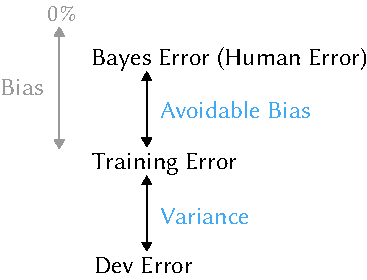
\includegraphics[width=6cm]{avoidable_bias.pdf}
    \caption{Avoidable Bias and Variance}
    \label{fig:avoidable_bias}
\end{figure}

\subsubsection{Understanding Human-level Performance}

在自然感知类任务上,例如图像分类、语音识别、文本分类等,
深度学习的方法很难达到人类的水平,人类的水平可以作为贝叶斯错误率的估计。
但在一些特定的任务上,例如广告推荐、搜索排序等,深度学习的方法已经超过了人类的水平,
在有大量数据的情况下,深度学习的方法可以达到很高的性能。

\subsubsection{Improving your Model Performance}

偏差大方差小说明模型拟合程度不足或训练不够充分;而偏差小方差大说明模型过拟合。

根据图~\ref{fig:avoidable_bias},确定可避免偏差和方差,并采取相应的措施:

\begin{enumerate}
    \item 如果可避免偏差较大,你可以尝试以下选项:
        \begin{itemize}
            \item 训练更大的模型。
            \item 使用更好的优化算法(如 Momentum、RMSprop、Adam)进行更长时间的训练。
            \item 寻找更好的神经网络架构/超参数搜索。
        \end{itemize}
    \item 如果方差较大,你可以尝试以下选项:
        \begin{itemize}
            \item 获取更多的训练数据。
            \item 正则化(如 L2、Dropout、数据增强)。
            \item 寻找更好的神经网络架构/超参数搜索。
        \end{itemize}
\end{enumerate}
